

\begin{theorem}
	Существует единственная мера $\nu$ на $\mathcal{A}_M$, такая что для любой параметризации $\phi : V \to U$ окрестности $U$ в $M$ и любого измеримого $A \subset U$ выполнено 
	\[ \nu(A) = \int_{\phi^{-1}(A)} \sqrt{g_{\phi}(x)} \, d \mu(x). \tag{$*$}\]
\end{theorem}

\begin{myproof}
	Определим $\nu$ на $\mathcal{A}_U$ по формуле $(*)$ и покажем, что она единственным образом продолжается на $\mathcal{A}_M$.
	Доказательство проведем в несколько шагов.

	\vspace{5pt}
	Покажем, что значение $\nu(A)$ определено корректно, то есть не зависит ни от координатной окрестности, содержащей $A$, ни от ее параметризации. 
	Пусть $\phi : V \to \R^n$, $\psi : W \to \R^n$ локальные параметризации, $A \subset O := \phi(V) \cap \psi(W)$.
	Тогда $\Phi = \psi^{-1} \circ \phi : \phi^{-1}(O) \to \psi^{-1}(O)$ является диффеоморфизмом. 
	Обозначим матрицу Якоби $\Phi$ через $S$, тогда, дифференцируя равенство $\phi = \psi \circ \Phi$, имеем 
	$D \phi = D \psi \cdot S$. Следовательно, $G_{\phi} = S^T G_{\psi} S$ и $g_{\phi} = g_{\psi} (\det S)^2$. 
	Теперь независимость следует из теоремы о замене переменных в кратном интеграле. 
	Действительно, при замене $y = \Phi(x)$ получим  
	\[ \int_{\psi^{-1}(A)} \sqrt{g_{\psi}(y)} \, d \mu(y) = \int_{\Phi^{-1}(\psi^{-1}(A))} \sqrt{g_{\psi} (\Phi(x))} \cdot |\det S| \, d \mu(x) = \int_{\phi^{-1}(A)} \sqrt{g_{\phi}(x)} \, d \mu (x). \]

	\vspace{5pt}
	Пусть семейство $\{E_i\}_{i=1}^{\infty}$ составляет измеримое разбиение $M$. 
	Для $A \in \mathcal{A}_M$ определим $A_i = A \cap E_i$. 
	Тогда каждое $A_i$ измеримо, лежит в образе некоторой параметризации и $A = \bigsqcup_{i=1}^{\infty} A_i$.
	Любая мера $\nu$ на $\mathcal{A}_M$, если существует, то удовлетворяет равенству $\nu(A) = \sum \limits_{i=1}^{\infty} \nu(A_i)$.
	Поскольку $\nu(A_i)$ определены однозначно, то $\nu(A)$ также определено однозначно. 
	Это дает способ продолжения $\nu$ с $\mathcal{A}_U$ на $\mathcal{A}_M$.

	\vspace{5pt}
	Осталось показать, что данная функция $\nu$ является мерой. 
	Достаточно показать счетную аддитивность, пусть $A = \bigsqcup_{k=1}^{\infty} B_k$. 
	Определим $B_{ki} = B_k \cap E_i$, $A_i = A \cap E_i$. Тогда 
	$B_k = \bigsqcup_{i=1}^{\infty} B_{ki}$, $A_i = \bigsqcup_{k=1}^{\infty} B_{ki}$. 
	Поскольку интеграл в формуле $(*)$ счетно аддитивен, то $\nu(A_i) = \sum \limits_{k=1}^{\infty} \nu(B_{ki})$ и $\nu(B_k) = \sum \limits_{i=1}^{\infty} \nu(B_{ki})$.
	Меняя порядок суммирования, получим 
	\[ \nu(A) = \sum \limits_{i=1}^{\infty} \nu(A_i) = \sum \limits_{i=1}^{\infty} \sum \limits_{k=1}^{\infty} \nu(B_{ki}) = \sum \limits_{k=1}^{\infty} \sum \limits_{i=1}^{\infty} \nu(B_{ki}) = \sum \limits_{k=1}^{\infty} \nu(B_k). \]
	В частности, показана независимость продолжения $\nu$ от выбора разбиения $\{E_i\}_{i=1}^{\infty}$. 
\end{myproof}


\begin{definition}
	Мера $\nu$ называется \textit{поверхностной мерой} на $M$.
\end{definition}

Относительно $\sigma$-алгебры $\mathcal{A}_M$ стандартным образом определяются измеримые функции.

\begin{definition}
	Пусть заданы $E \in \mathcal{A}_M$ и $f : E \to \overline{\R}$.
	Функция $f$ называется \textit{измеримой}, если $\forall a \in \R : \{p \in E : f(p) < a\} \in \mathcal{A}_M$.
\end{definition}

Следующая лемма позволяет проверять измеримость функции в координатах.

\begin{lemma}
	Пусть $E \in \mathcal{A}_M$ и $f : E \to \overline{\R}$. 
	Следующие условия эквивалентны: 
	\begin{enumerate}[itemsep = 0pt, topsep = 5pt]
		\item Функция $f$ измерима, 
		\item Функция $f \circ \phi$ измерима на $\phi^{-1}(E)$ для любой параметризации $\phi$, 
		\item Функция $f \circ \phi_j$ измерима на $\phi^{-1}_j(E)$ при любом $j$ для некоторого счетного набора параметризаций $\{\phi_j\}$, образы которых покрывают $M$.  
	\end{enumerate}
\end{lemma}

\begin{myproof}
	$(1 \Ra 2)$ Вытекает из равенства $\{x \in \phi^{-1}(E) : f(\phi(x)) < a\} = \phi^{-1} \{p \in E : f(p) < a\}$, так как в правой части прообраз $\phi^{-1}$ от измеримого множества.

	\vspace{5pt}
	$(2 \Ra 3)$ Это логически очевидно.

	\vspace{5pt}
	$(3 \Ra 1)$ Пусть $\{U_j\}_{j=1}^{\infty}$ -- набор координатных окрестностей, покрывающих $M$, для параметризаций $\phi_j : V_j \to U_j$. 
	Пусть $F = f^{-1}([-\infty, a))$. По равенству из первой импликации имеем: $\{x \in \phi^{-1}_j(E) : f(\phi_j(x)) < a\} = \phi_j^{-1}(F) = \phi_j^{-1}(F \cap U_j)$, то есть $\forall j : \phi^{-1}_j(F \cap U_j)$ измеримо. 
	Осталось применить первое замечание после определения измеримости.
\end{myproof}

\begin{definition}
	Пусть $f : A \to [0, +\infty]$ измерима, $\{E_i\}_{i=1}^{\infty}$ -- измеримое разбиение $M$, соответствующее набору параметризаций $\{\phi_i\}_{i=1}^{\infty}$.
	Определим \textit{интеграл Лебега по мере $\nu$}
	\[ \int_{A} f(x) \, d\nu(x) := \sum \limits_{i=1}^{\infty} \int_{\phi_{i}^{-1}(A \cap E_i)} (f \circ \phi_i)(y) \cdot \sqrt{g_{\phi_i}(y)} \, d\mu(y). \tag{$**$}\]
\end{definition}

\begin{note}
	Определение не зависит ни от измеримого разбиения $\{E_i\}$, ни от выбора параметризаций $\{\phi_i\}$:
	достаточно в доказательстве теоремы заменить $\sqrt{g_{\phi}}$ на $f \circ \phi \sqrt{g_{\phi}}$.
\end{note}

\begin{definition}
	Функция $f : A \to \overline{\R}$ называется \textit{интегрируемой}, если $f : A \to \overline{\R}$ измерима и $\int_{A} f^{\pm} \, d \nu < \infty$. 
	В этом случае $\int_A f \, d \nu = \int_A f^+ \, d \nu - \int_A f^- \, d \nu$.
\end{definition}

\begin{example}
	Пусть задан интервал $I \subset \R$ и гладкая кривая $\gamma : I \to \R^n$ с $\gamma'(t) \neq 0$ на $I$. 
	Если $\gamma : I \to \gamma(I)$ гомеоморфизм, то $\Gamma = \gamma(I)$ является гладким одномерным многообразием, покрываемым образом одной параметризации $\gamma$.
	Матрица Якоби $D \gamma$ -- столбец $\gamma'(t)$, $(D \gamma)^T D \gamma = |\gamma'(t)|^2$.
	Если $f : \Gamma \to \overline{\R}$ неотрицательная измеримая или интегрируемая функция, то интеграл $(**)$ примет вид ($ds := d\nu$):
	\[ \int_{\Gamma} f \, ds = \int_{I} f(\gamma(t)) \cdot |\gamma'(t)| \, dt. \]
	Этот интеграл называется \textit{криволинейным интегралом I-го рода}.
	В частности, если $\widetilde{\Gamma} = \gamma([a, b])$, то $\nu(\widetilde{\Gamma}) = \int_a^b |\gamma'(t)| \, dt$ совпадает с длиной кривой $\gamma$.
\end{example}

\begin{example}
	Пусть задано открытое $V \subset \R^2$ и отображение $r : V \to \R^n$ с $\operatorname{rk} Dr = 2$ на $V$. 
	Если $r : V \to r(V)$ гомеоморфизм, то $M = r(V)$ является гладким двумерным многообразием, покрываемым образом одной параметризации $r$. Матрица Якоби $Dr$ состоит из двух столбцов $r'_u, r'_v$, откуда
	\[ (Dr)^T Dr = \begin{pmatrix}
		(r'_u, r'_u) & (r'_u, r'_v) \\ 
		(r'_u, r'_v) & (r'_v, r'_v)
	\end{pmatrix} =: \begin{pmatrix}
		E & F \\ 
		F & G 
	\end{pmatrix}. \]
	Если $f : M \to \overline{\R}$ неотрицательная измеримая или интегрируемая функция, то интеграл $(**)$ примет вид ($dS := d\nu$):
	\[ \int_{M} f \, dS = \iint_{V} f(r(u, v)) \cdot \sqrt{EG - F^2} \, du \, dv. \]
	Этот интеграл называется \textit{поверхностным интегралом I-го рода}.
	В частности, площадь поверхности вычисляется по формуле $\nu(M) = \iint_V \sqrt{EG - F^2} \, du \, dv$.
\end{example}

\begin{example}
	Пусть задано открытое $U \subset \R^{n-1}$ и гладкая функция $h : U \to \R$, тогда $\Gamma_h = M = \{(x, h(x)) : x \in U\}$ является гладким $(n-1)$-мерным многообразием 
	в $\R^n$, покрываемым образом одной параметризации $\phi : U \to M$, $\phi(x) = (x, h(x))$. 
	Матрица Якоби $D \phi$ имеет блочный вид:
	\[ M_{n \times (n-1)} \ni D \phi = \begin{pmatrix}
		E_{n-1} \\ 
		(\nabla h)^T
	\end{pmatrix}, \]
	где $(\nabla h)^T$ -- строка частных производных $h$. 
	Имеем $G_{\phi} = E_{n-1} + \nabla h \cdot (\nabla h)^T$, тогда $\det G_{\phi}= 1 + |\nabla h|^2$ (в силу $
\left(\begin{smallmatrix} E & 0 \\ u^T & 1 \end{smallmatrix}\right)
\left(\begin{smallmatrix} E+uu^T & u \\ 0 & 1 \end{smallmatrix}\right)
\left(\begin{smallmatrix} E & 0 \\ -u^T & 1 \end{smallmatrix}\right)
=
\left(\begin{smallmatrix} E & u \\ 0 & 1+u^Tu \end{smallmatrix}\right)
$). 
	Если $f : M \to \overline{\R}$ неотрицательная измеримая или интегрируемая функция, то интеграл $(**)$ примет вид: 
	\[ \int_M f \, d\nu = \int_U f(x, h(x)) \sqrt{1 + |\nabla h(x)|^2} \, d\mu(x) = \int_U f(x, h(x)) \sqrt{1 + \sum_{i=1}^{n-1} \left(\frac{\partial h}{\partial x_i}(x)\right)^2} \, d\mu(x). \]
\end{example}

\begin{example}
	Пусть $M = \{x \in \R^n : |x| = r \wedge x_n > 0\}$ -- верхняя полусфера, тогда
	$M$ является графиком функции $h(y) = \sqrt{r^2 - |y|^2}$ над областью $U = B_r(0) = \{y : |y| < r\}$, где $y = (x_1, \dotsc, x_{n-1})$.
	Имеем $\frac{\partial h}{\partial x_i} = - \frac{x_i}{\sqrt{r^2 - |y|^2}}$, тогда $1 + \sum \limits_{i=1}^{n-1} \left( \frac{\partial h}{\partial x_i} \right)^2 = \frac{r^2}{r^2 - |y|^2}$, а значит, 
	\[ \int_{M} f \, d \nu = \int_{B_r(0)} f(y, \sqrt{r^2 - |y|^2}) \cdot \tfrac{r}{\sqrt{r^2 - |y|^2}} \, dy \overset{y = rt}{=} \int_{B_1(0)} f(rt, r \sqrt{1 - |t|^2}) \cdot \tfrac{r^{n-1}}{\sqrt{1 - |t|^2}} \, dt. \]
	В частности, $\nu(M) =  r^{n-1} \int_{B_1(0)} \frac{dt}{\sqrt{1 - |t|^2}} = r^{n-1} \cdot \nu(M_1)$, где $M_1$ -- единичная полусфера.
\end{example}


\begin{lemma}
	Пусть $A \in \mathcal{A}_M$. Следующие утверждения эквивалентны: 
	\begin{enumerate}[itemsep = 0pt, topsep = 5pt]
		\item $\nu(A) = 0$, 
		\item $\mu(\phi^{-1}(A \cap U)) = 0$ для любой параметризации $\phi : V \to U$, 
		\item $\mu(\phi_j^{-1}(A \cap U_j)) = 0$ для счетного набора параметризаций $\{\phi_j : V_j \to U_j\}$, образы $U_j$ которых покрывают $M$. 
	\end{enumerate}
\end{lemma}

 \begin{myproof}
	$(1 \Ra 2)$ Поскольку $A \cap U$ измеримо, то
	$0 = \nu(A) \geq \nu(A \cap U) = \int_{\phi^{-1}(A \cap U)} \sqrt{g_{\phi}} \, d \mu$. 
	Так как матрица Грама $(D \phi)^T D \phi$ положительно определена, $\operatorname{rk} D \phi$ максимален, то $\sqrt{g_{\phi}} > 0$ всюду, поэтому это возможно лишь при $\mu(\phi^{-1}(A \cap U)) = 0$.

	\vspace{5pt}
	$(2 \Ra 3)$ Это логически очевидно.

	\vspace{5pt}
	$(3 \Ra 1)$ Имеем $A = \bigcup_{j=1}^{\infty} (A \cap U_j)$. 
	По условию $\mu(\phi^{-1}_j(A \cap U_j)) = 0$, поэтому $\nu(A \cap U_j) = 0$ как интеграл по множеству меры нуль.
	В силу счетной аддитивности $\nu(A) = 0$.
 \end{myproof}


 \begin{corollary}
	Пусть $P \subset M$ -- гладкое $k$-мерное подмногообразие в гладком $m$-мерном многообразии $M$, где $k < m$. 
	Тогда $\nu(P) = 0$   
 \end{corollary}

 \begin{myproof}
	Зафиксируем $p \in P$. Рассмотрим параметризацию $\phi : V \subset \R^m \to U$ многообразия $M$ в окрестности этой точки.
	Прообраз $S = \phi^{-1}(P \cap U)$ будет гладким $k$-мерным подмногообразием в $V \subset \R^m$, так как у него есть сквозная параметризация через диффеоморфизм $\phi^{-1}$, как композиция с параметризацией $P$.
	Сузим $V$, тогда существует выпрямляющий диффеоморфизм $\Phi : V \to W$, такой что $\Phi(S) = W \cap (\R^k \times \{0\})$. 
	Рассмотрим новую параметризацию $\psi = \phi \circ \Phi^{-1} : W \to U$ многообразия $M$, тогда $\psi^{-1}(P \cap U) =  W \cap (\R^k \times \{0\})$. 
	Поскольку $k < m$, то $m$-мерная мера Лебега этого множества равна нулю. 
	Следовательно, $\nu(P) = 0$ по лемме, так как мы можем построить счетное число параметризаций $\psi$.
\end{myproof}

\vspace{-5pt}
\begin{figure}[h!]
\centering
\begin{framed}
		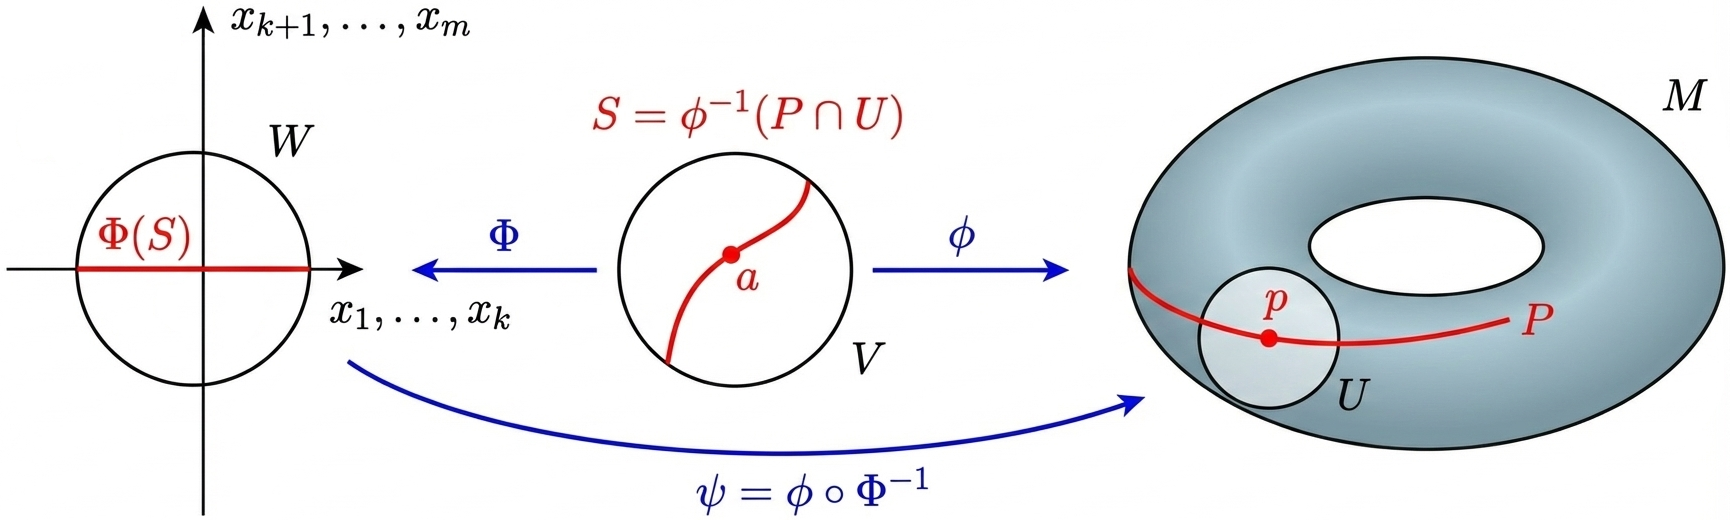
\includegraphics[width=0.8\textwidth, ]{Pictures/Lemma54.png}
		\label{fig:Lemma54}
\end{framed}
\end{figure}

\newpage

 \begin{definition}
	Множество $M \subset \R^n$ называется \textit{кусочно-гладким $m$-мерным многообразием}, если оно представимо в виде $N \cup (\bigcup_{i=1}^{\infty} P_i)$, где $N$ -- гладкое $m$-мерное многообразие, $P_i$ -- гладкие многообразия размерности строго меньше $m$.
 \end{definition}

 \begin{note}
	Для кусочно-гладкого многообразия $M$ мы доопределяем меру естественным образом, пренебрегая мерой множеств $P_i$.
 \end{note}
